\chapter{Quantum Monte-Carlo Methods} \label{chp:methods}
\epigraph{Great quote.}{Author}
\begin{figure}[H]
	\centering
	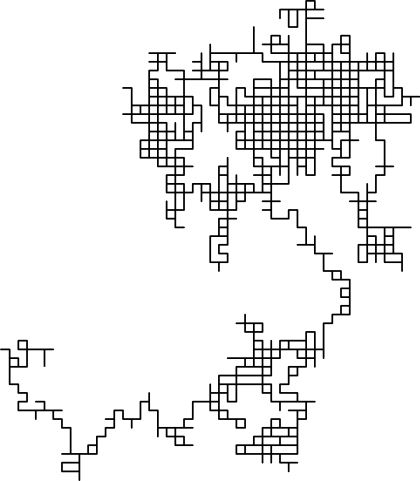
\includegraphics[scale=0.4]{Images/random_walk.png}
	\caption{Random walk in two dimensions on a grid.\\ © Copyright wikipedia.org.}
\end{figure}

Some great quantum many-body methods have been developed throughout the past century. The Hartree-Fock method is one of the most successful, which sets up a mean field and is thus relatively computational cheap to work with. It works also as an input to so-called post-Hartree-Fock methods, which includes configuration interaction, coupled cluster and quantum Monte-Carlo. The two former will be discussed in the next chapter, together with the Hartree-Fock method itself, and in this chapter we will dig into the quantum Monte-Carlo methods. 

Monte Carlo methods in quantum mechanics are a bunch of methods that are built on diffusion processes, and includes variational Monte Carlo (VMC), diffusion Monte Carlo (DMC) and others. The common denominator is that we move particles in order to find the optimal configuration, usually where the energy is minimized. Usually one uses the methods to study time-independent systems, but also time-dependent systems can be studied by for example time-dependent variational Monte-Carlo.

As variational Monte-Carlo is our main focus in this work, it will be explained thoroughly in this chapter together with common sampling tools. In the end, we will briefly explain the idea behind the diffusion Monte-Carlo method, which is in principle is capable of giving exact solutions of the Schrödinger equation. This methods will not be implemented, but since we will use it as our reference for most of the systems, it is natural to include a section on it.

\section{Variational Monte-Carlo} \label{subsec:vmc}
The variational Monte-Carlo (hereafter VMC) method is today widely used when it comes to the study of ground state properties of quantum mechanical systems. It makes use of Markov chain Monte-Carlo methods, often abbreviated MCMC, where the particles are assumed to be moving in Markov chains and Monte-Carlo simulations are used. The method has been used in studies of fermionic systems since the 1970's. \cite{deb_variational_2014} If we go back to the variational principle in equation \eqref{eq:variationalprinciple}, we see that by choosing a wave function which satisfies the criteria, we will get an energy larger or equal to the ground state energy. \bigskip

There are two main problems we need to solve
\begin{enumerate}
	\item We seldomly know the correct wave function
	\item The integral we need to find the energy is hard or impossible to solve analytically
\end{enumerate}
Let us first determine the last problem, which often is considered as the root of all evil. Solving this integral analytically is impossible, but we can approximate it with a sum,
\begin{align}
E &\leq \frac{\int d\bs{r}\Psi_T(\bs{r})^*\hat{\mathcal{H}}\Psi_T(\bs{r})}{\int d\bs{r}\Psi_T(\bs{r})^*\Psi_T(\bs{r})} \notag\\
& = \int P(\bs{r}) E_L(\bs{r}) d\bs{r} \notag\\
& \approx \frac{1}{M}\sum_{i=1}^ME_L(\bs{r}_i) \label{eq:energysum}
\end{align}
which is a common trick in statistical physics. The local energy is defined as
\begin{equation}
E_L(\bs{r})\equiv\frac{1}{\Psi_T(\bs{r})}\hat{\mathcal{H}}\Psi_T(\bs{r})
\label{eq:local energy}
\end{equation}
and the $\bs{r}_i$ is withdrawn from the probability distribution $P(\bs{r})$, which is given by
\begin{equation}
P(\bs{r})=\frac{|\Psi_T(\bs{r})|^2}{\int d\bs{r}|\Psi_T(\bs{r})|^2}.
\label{eq:probvmc}
\end{equation}
When increasing the number of energies drawn from the distribution, $M$, henceforth denoted as Monte-Carlo cycles, the standard error decreases and we get a more accurate energy. The error goes as $\mathcal{O}(1/\sqrt{M})$, and in the limit when $M$ goes to infinity, the error goes to zero,
\begin{equation}
\langle E_L\rangle=\lim_{M\to\infty} \frac{1}{M}\sum_{i=1}^ME_L(\bs{r}_i).
\end{equation}
This is associated with a zero-variance property, which is detailed in 
Zero-variance property: 
For more statistical details, see \cite{deb_variational_2014}. 

Generally, sampling from the beginning of the chain may not represent the desired distribution. Instead, we introduce a \textit{burn-in period}, which does not contribute to the expectation values. The burn-in period is associated with a equilibriation fraction, which how big amount of the total cycles that should be in the burn-in period. When running multiple parallel processes, the burn-in period should be the same at all the processes.

We also have a technique called \textit{thinning}, which means picking every $n$'th sample in the chain and ignore the rest. This 

So far, so good, but how about the first problem stated above? How do we find the correct wave function? In VMC, we define a wave function with variational parameters, which are adjusted in order to minimize the energy for every iteration. Of course, we need a decent initial guess, which is usually based on our physical intuition. We will later examine how much physical intuition we need to get an acceptable result. 

For every iteration, we run $M$ Monte-Carlo cycles where we withdraw a new position $\bs{r}_i$. Whether or not the proposed move should be accepted is determined by a Markov chain Monte-Carlo method, as for instance the Metropolis method. In the following we will explain how it works and present an algorithm for it.

\section{The Metropolis algorithm}
Metropolis sampling is a Markov chain Monte-Carlo method, which generates a Markov chain using a proposal density for new steps, and the method also rejects unsatisfying moves. In its most simple form, a particle is moved in a random direction, which was the original method invented by Metropolis et.al. back in 1953. \cite{metropolis_equation_1953} Later, the method was improved by Hastings et.al., giving rise to the more general Metropolis-Hastings algorithm. \cite{hastings_monte_1970}
The genius of the Metropolis algorithm, is that the acceptance of a move is not based on the probabilities themselves, but the ratio between the new and the old probabilities. In that way, we avoid calculating the sum over all probabilities, which is often computational intractable.

We will first discuss Markov chains in general, before we connect them to the original Metropolis algorithm, henceforth called \textit{brute-force sampling}, and then the Metropolis-Hastings algorithm, also called \textit{importance sampling}.

If we denote $\bs{r}$ as the current state, and $\bs{r}'$ as the proposed state, we have a transition rule $P(\bs{r}'|\bs{r})$ for going from $\bs{r}$ to $\bs{r}'$ and a transition rule $P(\bs{r}|\bs{r}')$ for going the opposite way. If we then assume that the rules satisfy \textit{ergodicity} and \textit{detailed balance}, we have the following relationship:
\begin{equation}
P(\bs{r}'|\bs{r})P(\bs{r})=P(\bs{r}|\bs{r}')P(\bs{r}'),
\end{equation}
which is actually a restatement of Bayes' theorem presented in section \ref{sec:bayes}.

The next step is to rewrite the transition rules in terms of a proposal distribution $T(\bs{r}'|\bs{r})$ and an acceptance probability $A(\bs{r}',\bs{r})$,
\begin{equation}
P(\bs{r}'|\bs{r})=T(\bs{r}'|\bs{r})A(\bs{r}',\bs{r}).
\end{equation}
In order to satisfy the detailed balance, we need to choose $A(\bs{r}',\bs{r})$ such that
\begin{equation}
A(\bs{r}',\bs{r})=\text{min }\left[1,\frac{T(\bs{r}|\bs{r}')P(\bs{r}')}{T(\bs{r}'|\bs{r})P(\bs{r})}\right],
\label{eq:acceptance}
\end{equation}
since $A$ cannot be larger than 1. We want to accept a move with probability $A(\bs{r}',\bs{r})$. One way to do that is to draw a number from a uniform distribution between 0 and 1. If this number is lower than the acceptance, the move should be accepted. Otherwise it will be rejected.

\subsection{Brute-force sampling}
In its simplest form, the move is proposed randomly both in magnitude and direction. Mathematically, we can write this as
\begin{equation}
\bs{r}'=\bs{r}+sd\bs{r}
\end{equation}
where $s$ is a random number which determines the distance to move and $d\bs{r}$ is a random direction (typically which particle to move). We obtain the naive acceptance probability when requiring $T(\bs{r}'|\bs{r})=T(\bs{r}|\bs{r}')$, such that the it simplifies to
\begin{equation}
A(\bs{r}',\bs{r})=\text{min }\left[1,\frac{P(\bs{r}')}{P(\bs{r})}\right].
\end{equation}

However, with this approach a lot of moves will be rejected, which results in a significant waste of computing power. A better method is \textbf{importance sampling}.

\subsection{Importance sampling} \label{sec:importancesampling}
Importance sampling is a more intelligent sampling method than the brute-force sampling, since the new position is based on an educated guess. To understand how it works, we need to take a quick look at diffusion processes. We start from the Fokker-Planck equation,
\begin{equation}
\frac{\partial P(\bs{r},t)}{\partial t}=D\nabla\left(\nabla-\bs{F}\right)P(\bs{r},t)
\end{equation}
which describes how a probability distribution $P(\bs{r},t)$ evolves in appearance of a drift force $\bs{F}$. In the case $\bs{F}=0$, the equation reduces to the diffusion equation with $D$ as the diffusion constant. This simplifies to $D=1/2$ in atomic units. 

The Langevin equation states that a diffusion particle tends to move parallel to the drift force in the coordinate space, but because of a random variable $\bs{\eta}$ this is not always true. The equation reads
\begin{equation}
\frac{\partial \bs{r}(t)}{\partial t}=D\bs{F}(\bs{r}(t))+\bs{\eta}.
\label{eq:langevin}
\end{equation}
Given a position $\bs{r}$, the new position $\bs{r}'$ can be be found by applying forward-Euler on equation \eqref{eq:langevin},
\begin{equation}
%\bs{r}'=\bs{r}+D\bs{F}(\bs{r})\Delta t + \bs{\xi}\sqrt{\Delta t}
\end{equation}
where $\Delta t$ is a fictive time step and $\bs{\xi}$ is a Gaussian random variable. The next thing we want to find, is an expression for the drift force $\bs{F}$ which makes the system converge to a stationary state. 

A stationary state is found when the probability density $P(\bs{r})$ is constant in time, i.e, when the left-hand-side of Fokker-Planck is zero. In that case, we can write the equation as
\begin{equation}
\nabla^2P(\bs{r})=P(\bs{r})\nabla\bs{F(\bs{r})}+\bs{F(\bs{r})}\nabla P(\bs{r}).
\end{equation}
In the next, we assume that the drift force takes the form $\bs{F(\bs{r})}=g(\bs{r})\nabla P(\bs{r})$, since the force should point to a higher probability. We can then go further and write
\begin{equation}
\nabla^2 P(\bs{r})\big(1-P(\bs{r})g(\bs{r})\big)=\nabla\big(g(\bs{r})P(\bs{r})\big)\nabla P(\bs{r})
\end{equation}
which is satisfied when $g(\bs{r})=1/P(\bs{r})$. We then get the drift force 
\begin{equation}
\bs{F}(\bs{r})=\frac{\nabla P(\bs{r})}{P(\bs{r})}=2\frac{\nabla\Psi_T(\bs{r})}{\Psi_T(\bs{r})}=2\nabla\ln\Psi_T(\bs{r}),
\end{equation}
which is also known as the \textit{quantum force}.

\IncMargin{1em}
\begin{algorithm} [t]
	\SetAlgoLined
	\Parameter{$\Delta t$: Fictive time step}
	\Data{$\bs{r}'$: Initial particle positions}
	\Require{$\Psi_T(\bs{r})$: Initial trial wave function guess}
	\BlankLine
	$\bs{F}(\bs{r}')\leftarrow2(\nabla\Psi_T(\bs{r}'))/\Psi_T(\bs{r}')$ (Initialize the quantum force) \;
	$p(\bs{r}',\bs{r})\leftarrow1$ (Initialize the probability ratio) \;
	$g(\bs{r}',\bs{r},\Delta t)\leftarrow1$ (Initialize Green's function ratio) \;
	\While{not converged}{
		$\bs{r}\leftarrow\bs{r}'$ (Save current positions $\bs{r}'$ in a vector $\bs{r}$) \;
		$\bs{F}(\bs{r})\leftarrow\bs{F}(\bs{r}')$ (Save the current quantum force, $\bs{F}(\bs{r}')$, in a vector $\bs{F}(\bs{r})$) \;
		$p(\bs{r},\bs{r}')\leftarrow p(\bs{r}',\bs{r})$ (Save current probability ratio)\;
		$g(\bs{r},\bs{r}',\Delta t)\leftarrow g(\bs{r}',\bs{r},\Delta t)$ (Save the current Green's function ratio) \;
		\BlankLine
		$\bs{r}'\leftarrow\bs{r}+D\Delta t\bs{F}(\bs{r}) + \bs{\xi}\sqrt{\Delta t}$ (Update position based on the Langevin equation) \;
		$\bs{F}(\bs{r}')\leftarrow2\nabla\ln\Psi_T(\bs{r'})$ (Update the quantum force) \;
		$p(\bs{r}',\bs{r})=|\Psi_T(\bs{r}')|^2/|\Psi_T(\bs{r})|^2$ (Update the probability ratio) \;
		$g(\bs{r}',\bs{r},\Delta t)=G(\bs{r}',\bs{r},\Delta t)/G(\bs{r},\bs{r}',\Delta t)$ (Update the Green's function ratio) \;
		$w\leftarrow p(\bs{r}',\bs{r}) g(\bs{r}',\bs{r},\Delta t)$ (Calculate acceptance probability) \;
		$q\leftarrow\mathcal{U}(0,1)$ (Draw a random number between 0 and 1)\;
		\eIf{$w<q$}{
			$\bs{r}'\leftarrow\bs{r}$ (Reset positions)\;
			$\bs{F}(\bs{r}')\leftarrow\bs{F}(\bs{r})$ (Reset the quantum force) \;
			$p(\bs{r}',\bs{r})\leftarrow p(\bs{r},\bs{r}')$ (Reset the probability ratio)\;
			$g(\bs{r}',\bs{r},\Delta t)\leftarrow g(\bs{r},\bs{r}',\Delta t)$ (Reset the Green's function ratio) \;
		}
		{
			keep going\;
		}
	}
	\KwResult{The optimized trial wave function.}
	\caption{The Metropolis-Hastings algorithm. The positions are initialized randomly or was chosen by a previous sampling. The parameters are also usually initialized randomly or chosen by a parameter update. The Green's function ratio, $g$, can be evaluated efficiently using equation \eqref{eq:greensratio}, and the probability ratio $p$ can also often be found in a simple closed-form expression. The diffusion constant is $D=1/2$ in natural units. $\bs{\xi}$ is a random Gaussian variable. For more information, see section \ref{sec:importancesampling}}.
	\label{alg:hastings}
\end{algorithm}\DecMargin{1em}

The remaining part is how to decide if a proposed move should be accepted or not. For this, we need to find the sampling distributions $T(\bs{r}'|\bs{r})$ from equation \eqref{eq:acceptance}, which are just the solutions of the Fokker-Planck equation. The solutions read
\begin{equation}
G(\bs{r},\bs{r}',\Delta t)\propto\exp\Big(-\big(\bs{r}-\bs{r}'-D\Delta t\bs{F}(\bs{r})\big)^2/4D\Delta t\Big)
\end{equation}
which is called Green's functions. They correspond to the normal distribution $\mathcal{N}(\bs{r}|\bs{r}'+D\Delta t \bs{F}(\bs{r}),2D\Delta t)$. The acceptance probability for importance sampling can finally be written as
\begin{equation}
A(\bs{r}'|\bs{r})=\text{min }\left[1,\frac{G(\bs{r},\bs{r}',\Delta t)P(\bs{r}')}{G(\bs{r}',\bs{r}, \Delta t)P(\bs{r})}\right],
\end{equation}
where the marginal probabilities are still given by equation \eqref{eq:probvmc}. 

As a summary, we set up the actual algorithm, known as Metropolis-Hasting's algorithm, see algorithm \eqref{alg:hastings}. In that algorithm, we write the position update in a general form, where we allow updating all the particles at the same time. However, often one ends up moving only a particle at each time step, as this make some advantageous optimization schemes possible. 

The ratio between the new and old Green's function can be expressed in the elegant form 
\begin{equation}
g(\bs{r}',\bs{r},\Delta t)\equiv\frac{G(\bs{r}',\bs{r},\Delta t)}{G(\bs{r},\bs{r}',\Delta t)}=\exp((\bs{r}'-\bs{r})\cdot(\bs{F}(\bs{r})-\bs{F}(\bs{r}'))/2)
\label{eq:greensratio}
\end{equation}
which can be evaluated very efficiently. Also the probability ratios can be computed in an efficient way for many trial wave functions $\Psi_T(\bs{r})$, in particular when the wave function is on an exponential form. In chapter \ref{chp:WFE}, we find closed-form expressions for
\begin{equation}
p(\bs{r}',\bs{r})\equiv\frac{P(\bs{r}')}{P(\bs{r})}=\frac{|\Psi_T(\bs{r}')|^2}{|\Psi_T(\bs{r})|^2}
\end{equation}
for all the wave function elements of interest, also the elements based on restricted Boltzmann machines. Additionally, closed-form expressions fo $\nabla\ln\Psi_T(\bs{r})$ are found, which are needed for the quantum force computations as well as the kinetic energy computations. 

\subsection{Gibbs sampling}
In the machine learning community, Gibbs sampling is widely used when it comes to training Boltzmann machines. It is popular partly because it does not require any "tuning". It is an instance of the Metropolis-Hastings algorithm, and is therefore another Markov chain Monte-Carlo method. In the Metropolis sampling, we have seen that some moves will be rejected, but in Gibbs sampling all the moved are accepted, which means that the we do not "waste" computations. 

The point of Gibbs sampling is that given a multivariate distribution it is simpler to sample from a conditional distribution than to marginalize by integrating over a joint distribution. This is the reason why we do not need the marginal distributions in Gibbs sampling, but rather the conditional distributions. In the most general, Gibbs sampling proposes a rule for going from a sample $\bs{x}^{(i)}=(x_1^{(i)},x_2^{(i)},\hdots,x_n^{(i)})$ to another sample $\bs{x}^{(i+1)}=(x_1^{(i+1)},x_2^{(i+1)},\hdots,x_n^{(i+1)})$, similar to the Metropolis algorithm. However, in Gibbs sampling the transition from $x_j^{(i)}$ to $x_j^{(i+1)}$ is performed according to the conditional distribution specified by
\begin{equation}
P\big(x_j^{(i+1)}|x_1^{(i+1)},\hdots,x_{j-1}^{(i+1)},x_{j+1}^{(i)},\hdots,x_n^{(i)}\big).
\end{equation}
The marginal distribution of a subset of variables can then be approximated by simply considering the samples for that subset of variables, ignoring the rest. 

For a restricted Boltzmann machine, this is a two-step sampling process, because of the latent variables, we use the conditional probabilities $P(\bs{r}|\bs{h})$ and $P(\bs{h}|\bs{r})$ to update the visible and hidden units respectively. For the restricted Boltzmann machine with Gaussian-binary units presented in section \ref{sec:RBM}, the conditional probability of $h_j=0$ given a set of visible nodes $\bs{x}$ is
\begin{equation}
P(h_j=0|\bs{x})=\frac{1}{1+\exp(b_j+\sum_{i=1}^Nx_iw_{ij}/\sigma^2)}
\end{equation}
and the corresponding conditional probability of $h_j=1$ is
\begin{equation}
P(h_j=1|\bs{x})=\frac{1}{1+\exp(-b_j-\sum_{i=1}^Nx_iw_{ij}/\sigma^2)},
\end{equation}
which is by the way the sigmoid function again. Note that $P(h_j=0|\bs{x})+P(h_j=1|\bs{x})=1$, indicating that a hidden node $h_j$ can only take 0 or 1, hence binary. When updating the hidden node, one typically calculate the sigmoid $P(h_j=1|\bs{x})$ and set $h_j$ to 1 if this probability is larger than 1/2, and set it to 0 otherwise. 

For the update of the visible nodes, we see from equation \eqref{eq:normal} that the visible nodes are chosen after the normal distribution,
\begin{equation}
P(x_i|\bs{h})=\mathcal{N}\Big(a_i+\sum_{j=1}^Hw_{ij}h_j,\sigma^2\Big)
\end{equation}
which introduce some stochasticity to the system. By going back and forth in the Boltzmann machine multiple times (a round trip corresponds to an iteration), the hope is that the expectation values can be approximated by averaging over all the iterations. 

As pointed out earlier, the Gibbs sampling will not be implemented in this work, but is described for completeness purposes. The reason for this, is that the method has not shown promising results for our specific problem, and we will instead rely on Metropolis sampling. We have already tested the Gibbs sampling in another similar project on small quantum dots \cite{nordhagen_computational_2018}, and so have others like Vilde Flugsrud \cite{flugsrud_vilde_moe_solving_nodate}. The results are similar and poor compared to the Metropolis-Hastings algorithm.

However, the Gibbs sampling method itself should not be underestimated. Carleo and Troyer showed its importance when solving the Ising model using a restricted Boltzmann machine and Gibbs sampling, and in traditional Boltzmann machines the Gibbs sampling is the preferred tool. \cite{carleo_solving_2017}

\section{Similarities between restricted Boltzmann machines and variational Monte-Carlo}
In chapter \ref{chp:systems}, we presented the relation between a quantum system and expressions of the Hamiltonian, which is the energy operator. In section \ref{sec:unsupervised}, we described how Boltzmann machines are defined and how one can find the energy of a Boltzmann machine. Further, we looked at the updating schemes, which for both cases corresponds to minimizing the cost function and maximizing the log-likelihood function. 

All in all, there are many similarities between the two methods. They are fundamentally related through Markov random fields, ...

\section{Diffusion Monte-Carlo}
Diffusion Monte-Carlo belongs to a class of projection and Green's function approaches. Consider the time-imaginary Schrödinger equation
\begin{eqnarray}
-\frac{\partial\Psi(\bs{r},\tau)}{\partial\tau}=(\mathcal{H}-E_T)\Psi(\bs{r},\tau)
\end{eqnarray}
where $\tau$ is the imaginary time and $E_T$ is an energy offset. If we first look at the equation with non-interacting particles, it contains basically only the kinetic energy term, 
\begin{equation}
\frac{\partial\Psi(\bs{r},\tau)}{\partial\tau}=\frac{1}{2}\nabla^2\Psi(\bs{r},\tau)
\end{equation}
which is really similar to the diffusion equation,
\begin{equation}
\frac{\partial\phi(\bs{r},t)}{\partial t}=D\nabla^2\phi(\bs{r},t)
\end{equation}
where $D$ is the diffusion constant set to $1/2$ in our calculations, no wonder why. The similarities between the imaginary time Schrödinger and the diffusion equation was noticed by Fermi already around 1945, and is what diffusion Monte-Carlo is based on \cite{metropolis_monte_1949,ceperley_quantum_1986}. 


